\chapter{Evaluations}\label{chap:eval}

\newcommand{\round}[1]{\DTLround{#1}{#1}{4}#1}

\section{Evaluation, the rationale}

As discussed in Chapter 2, we need to evaluate the quality of the data we extracted. \cite{ochoa2006} suggest a number of quality metrics, in this project, we will use Data Completeness, Data Accuracy, User perceived data quality and Conformance to Expectation (Data fitness) to evaluate our work. The reason for choosing them is because: 

\begin{description}
	\item \textbf{Data Completeness} can reflect how complete the LinkedIn profile is. It's an important statistics we can get from LinkedIn.com as people always interest in how complete for these profiles in general. It also a hint for future research since we can quickly identify sparse data fields and intensive data fields.
	\item \textbf{Data Accuracy} is where we introduce volunteers to manually extract the data out from the HTML files and ask them to rate our results from 1 to 5. By calculating prediction precisions, recalls, f-measures (will be discussed later) and user average ratings, we can know how well our parser and our data normalisation is.
	\item \textbf{User Perceived Data Quality} is simplified version of Data Accuracy. We present our results and show the user extracted resutls, then ask user rate our result from 1 to 5. As precision, recall and f-measure are too complex for people who do not have mathematic background, simple ratings can be more user friendly.
	\item \textbf{Data fitness} is to measure how well our knowledge model and our dataset match the requirements of the upper layer user interface. In this part, we collect feedbacks from the developer of the Data Visualisation project, and the drawbacks will be presented in our future works.
\end{description}

\subsection{Data completeness}

In this section, we present the completeness of profiles in LinkedIn.com. Researchers who also interested in LinkedIn.com public profiles can use this statistics as a measure, to avoid the fields that are too sparse.

Table~\ref{tab:NumCount} shows the total number of personal profiles, company profiles and total number of skills in all of the profiles. These numbers are base numbers that will be used to calculate the percentage in the following tables.

\begin{table}[H]
    \begin{tabular}{|c|c|}
    \hline
    Total number of public personal profiles & 13014 \\ \hline
    Total number of company profiles         & 24778 \\ \hline
    Total number of skills                   & 15917 \\ \hline
    \end{tabular}
    \caption{Total number of personal profiles, company profiles and skills}
  	\label{tab:NumCount}
\end{table}

\subsubsection{Public personal profile completeness}

Many people do not fill their complete work experiences and education backgrounds into LinkedIn, therefore, in our 13014 randomly download and selected profiles, we can have an overview of the percentage of people have sections that are missing.

\begin{table}[H]
    \begin{tabular}{|c|c|c|}
    \hline
    ~                                                             & Number & Percentage(of personal profiles) \\ \hline
    Profiles that have work experiences                           & 11501  & 88.4\%                             \\ \hline
    Profiles that have education                                  & 9913   & 77\%                               \\ \hline
    Profiles that have skills                                     & 10511  & 80\%                               \\ \hline
    Profiles that have city information & 10158  & 78\%                               \\ \hline
    Profiles that have academic degree information                & 5230   & 40.2\%                             \\ \hline
    Profiles that have college major information                  & 7825   & 60.1\%                             \\ \hline
    \end{tabular}
\end{table}

\subsubsection{Company profile completeness}

Not every company will register in LinkedIn company to have a company profile. If a company in a person's work experience registered on LinkedIn.com, there's a hyperlink that link the company name to the complete company profile. If the company is not registered, there will be not such hyperlink. So we can easily draw a conclusion from Table~\ref{tab:ComPercent}, around 46\% of companies in Ireland register in LinkedIn.com.

\begin{table}[H]
    \begin{tabular}{|c|c|c|}
    \hline
    ~                                            & Number & Percentage(of company profiles) \\ \hline
    Company profiles that have industry type     & 11868  & 47.9\%                             \\ \hline
    Company profiles that have organisation type & 11351  & 45.8\%                             \\ \hline
    Company profiles that have company size info & 11343  & 45.8\%                             \\ \hline
    \end{tabular}
    \caption{Company profile completeness}
    \label{tab:ComPercent}
\end{table}

\subsubsection{Data linkage}

The definition of RDF data linkage is: average\_linkage=$\frac{total\_number\_of\_links}{total\_number\_of\_objects}$. It's a measurement of how ``sparse'' of the RDF data is. Generally, high linkage means high correlation between objects.

\begin{table}[H]
    \begin{tabular}{|c|c|}
    \hline
    Total number of objects & 160251 \\ \hline
    Total number of links   & 415916 \\ \hline
    Average linkage                 & 2.595  \\ \hline
    \end{tabular}
\end{table}

\subsection{Data Accuracy (extracted metadata quality)}

\subsubsection{Evaluation setup}

We recruited 10 users, divided them into 5 groups, so each group have 2 participants. Each group of users will view same 10 randomly selected profiles. They were asked to manually extract city, work experiences (including company names, job titles, job start dates and job end dates) and education backgrounds (including college names, majors, degrees, college start dates, college end dates).

Then after the user fill in the data, we display what they entered as well as what we automatically extracted data, and ask them to rate our results, from 1 to 5, where score 5 is highest.

Below are the screenshots for the user interfaces:

\begin{figure}[H]
	\centering
	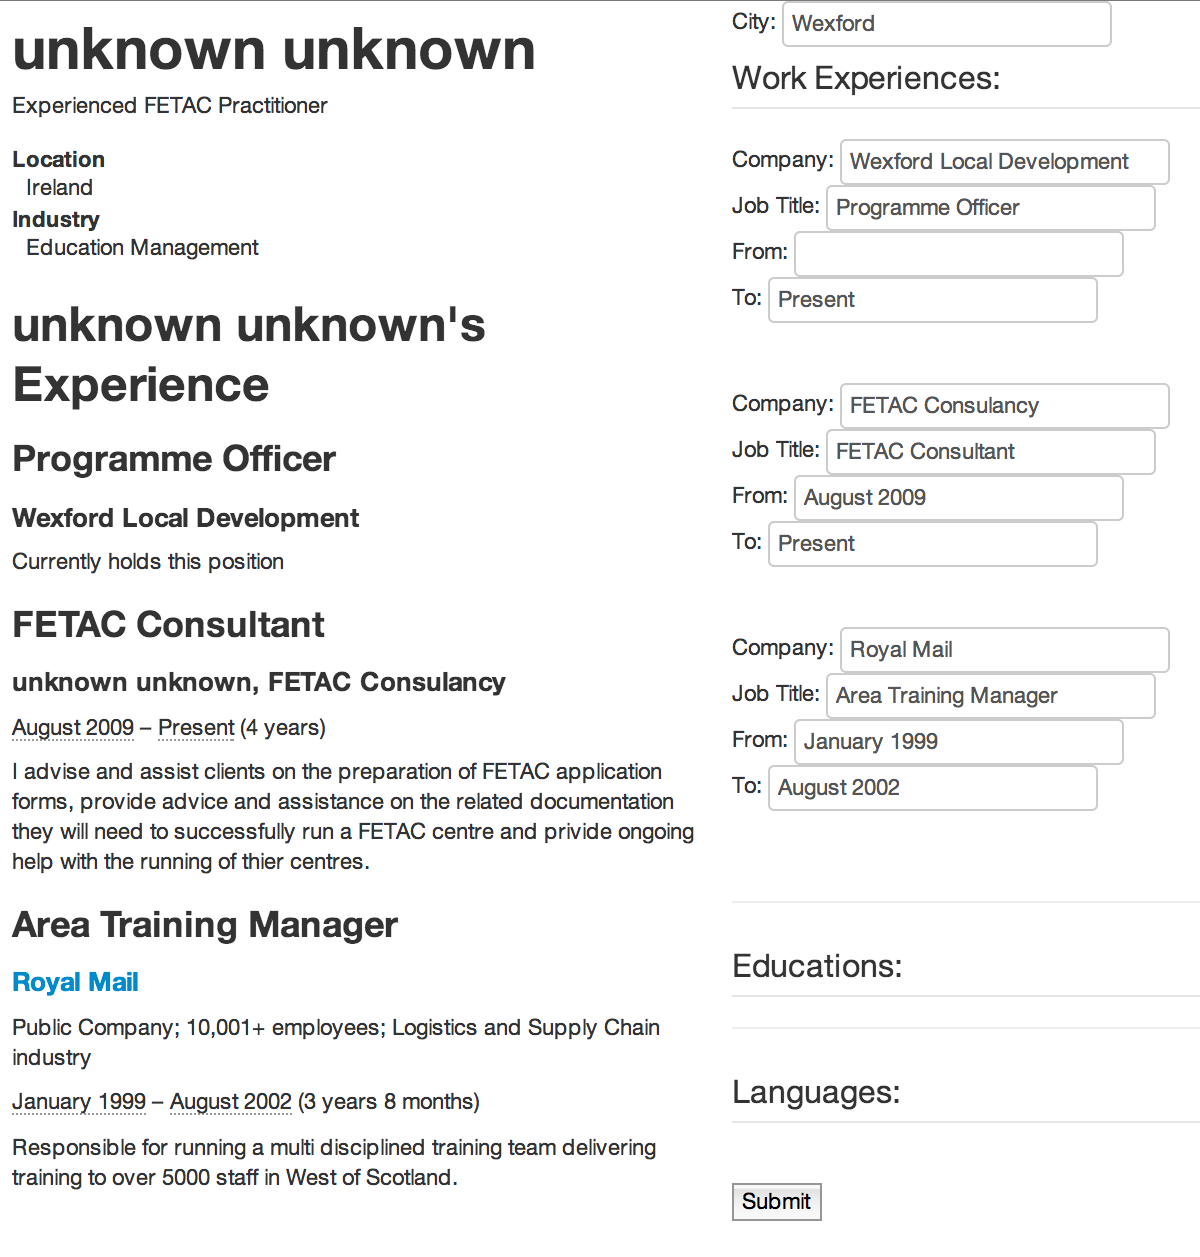
\includegraphics[width=1.0\textwidth]{images/user-input.png}
	\caption{Online user evaluation website: User manually extracted data\protect}
	\label{fig:UserInput}
\end{figure}

\begin{figure}[H]
	\centering
	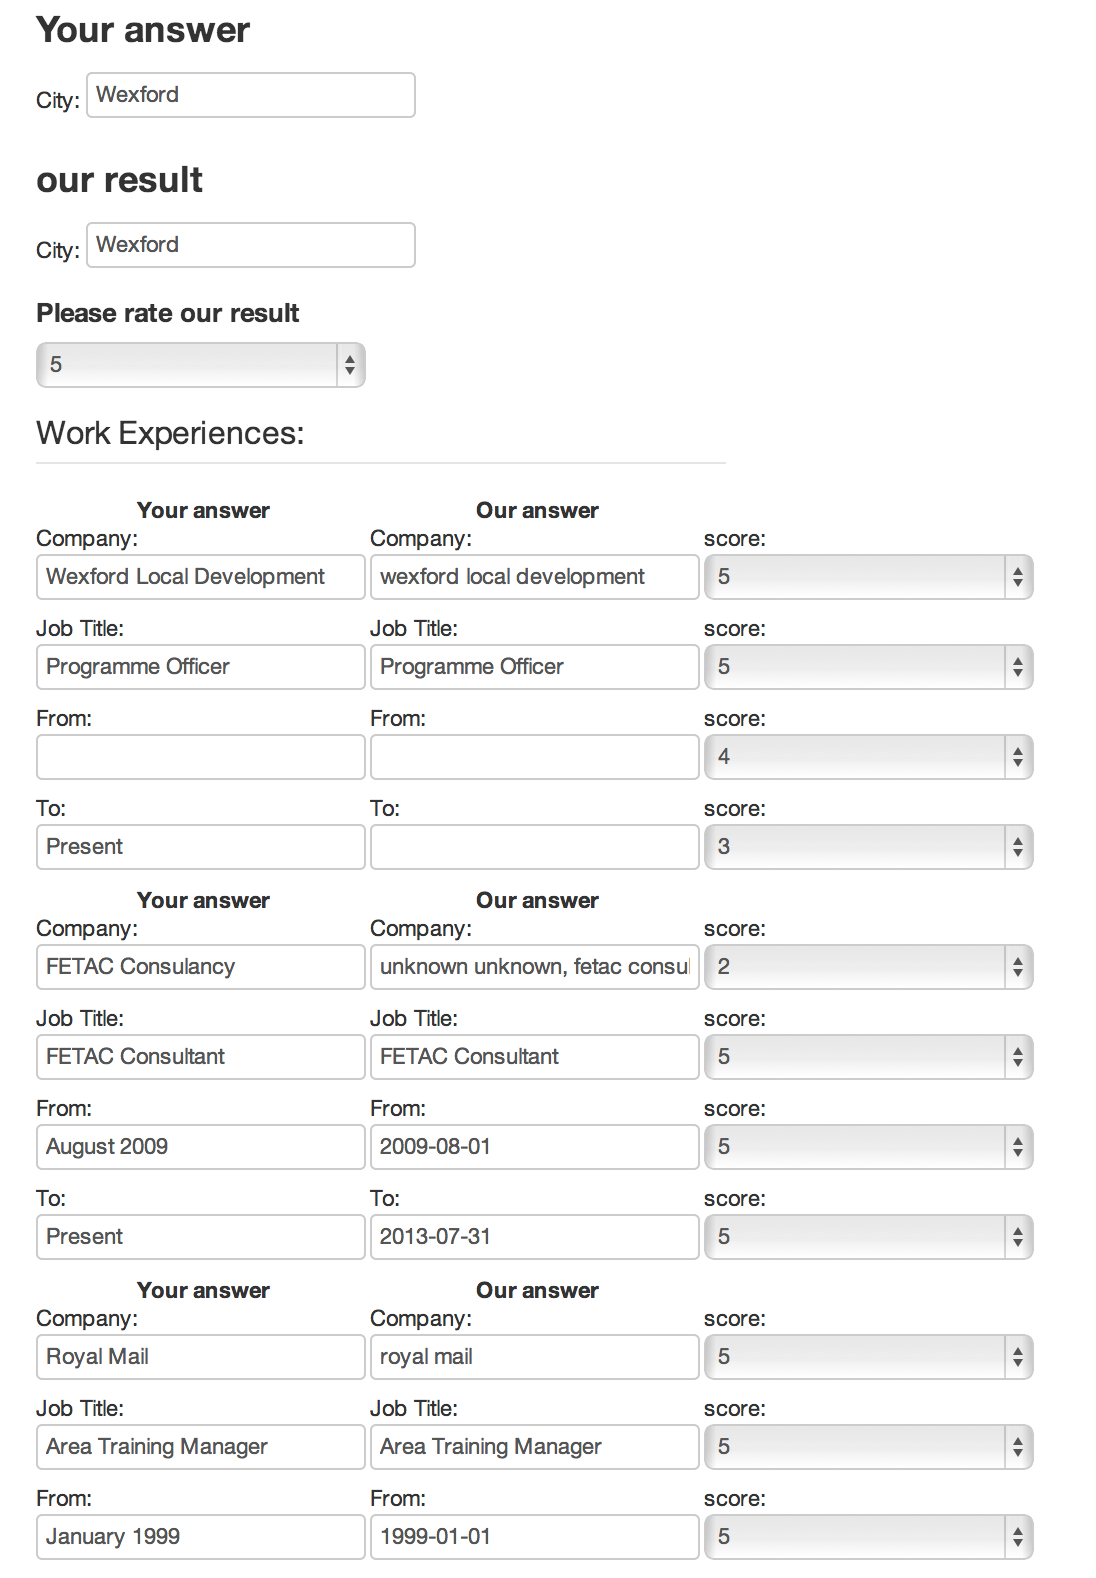
\includegraphics[scale=0.8]{images/user-compare.png}
	\caption{Online user evaluation website: Asking user compare manually extracted data with automatically extracted data\protect}
	\label{fig:UserCompare}
\end{figure}

\subsubsection{Results}

After the user evaluation, we take user input as the ground truth, we use string matching to compare entered data with automatic extracted data. If the string matching return false, we manually examine the data and decide whether the extracted data is correct.

The metrics here we use are precision, recall and f-measure.
\begin{equation}\label{eq:precision}
	precision=\frac{correctly\_predicted}{predicted}
\end{equation}
\begin{equation}\label{eq:recall}
	recall=\frac{correctly\_predicted}{total}
\end{equation}
\begin{equation}\label{eq:fmeasure}
	f-measure=\frac{2 * precision * recall }{precision + recall}
\end{equation}

The meaning of these metrics can be explained as follows\cite{powers2011evaluation}: Precision, or confidence, is focus on how good we are predicting; Recall, or sensitivity is a measure of the proportion we correctly predicted over total data size. F-measure, or F-score is designed to capture both precision and recall. In order to get high F-score, precision and recall must be high.

\begin{table}[H]
	\centering
	\DTLloaddb[keys={user,precision,recall,fmeasure}]{citycsv}{csvs/city.csv}
	\caption{Precision, recall and f-measure scores for city information}
	\begin{tabular}{|c|c|c|c|}
	\toprule \hline 
	\bfseries User & \bfseries Precision & \bfseries Recall & \bfseries F-Measure
	\DTLforeach{citycsv}{\user=user, \precision=precision, \recall=recall, \fmeasure=fmeasure}{%
	\ifthenelse{\value{DTLrowi}=1}{\tabularnewline \hline}{\tabularnewline \hline}
	\user & \round{\precision} & \round{\recall} & \round{\fmeasure} } \\
	\hline \bottomrule
	\end{tabular}
	\label{tab:cityResult}
\end{table}

According to the score, users are quite satisfy with our city information extraction strategy. Despite the fact that some lazy volunteer didn't fill in the ground truth, we still getting average of 0.85 F-score. It's acceptable for us to do complex query using person's city information.

\begin{table}[H]
	\centering
	\DTLloaddb[keys={user,precision,recall,fmeasure}]{companycsv}{csvs/company.csv}
	\caption{Precision, recall and f-measure scores for company information}
	\begin{tabular}{|c|c|c|c|}
	\toprule \hline 
	\bfseries User & \bfseries Precision & \bfseries Recall & \bfseries F-Measure
	\DTLforeach{companycsv}{\user=user, \precision=precision, \recall=recall, \fmeasure=fmeasure}{%
	\ifthenelse{\value{DTLrowi}=1}{\tabularnewline \hline}{\tabularnewline \hline}
	\user & \round{\precision} & \round{\recall} & \round{\fmeasure}} \\
	\hline \bottomrule
	\end{tabular}
	\label{tab:companyResult}
\end{table}

\begin{table}[H]
	\centering
	\DTLloaddb[keys={user,precision,recall,fmeasure}]{jobtitlecsv}{csvs/job_title.csv}
	\caption{Precision, recall and f-measure scores for job title information}
	\begin{tabular}{|c|c|c|c|}
	\toprule \hline 
	\bfseries User & \bfseries Precision & \bfseries Recall & \bfseries F-Measure
	\DTLforeach{jobtitlecsv}{\user=user, \precision=precision, \recall=recall, \fmeasure=fmeasure}{%
	\ifthenelse{\value{DTLrowi}=1}{\tabularnewline \hline}{\tabularnewline \hline}
	\user & \round{\precision} & \round{\recall} & \round{\fmeasure}} \\
	\hline \bottomrule
	\end{tabular}
	\label{tab:jobtitleResult}
\end{table}

\begin{table}[H]
	\centering
	\DTLloaddb[keys={user,precision,recall,fmeasure}]{experiencefromcsv}{csvs/experience_from.csv}
	\caption{Precision, recall and f-measure scores for experience start date information}
	\begin{tabular}{|c|c|c|c|}
	\toprule \hline 
	\bfseries User & \bfseries Precision & \bfseries Recall & \bfseries F-Measure
	\DTLforeach{experiencefromcsv}{\user=user, \precision=precision, \recall=recall, \fmeasure=fmeasure}{%
	\ifthenelse{\value{DTLrowi}=1}{\tabularnewline \hline}{\tabularnewline \hline}
	\user & \round{\precision} & \round{\recall} & \round{\fmeasure}} \\
	\hline \bottomrule
	\end{tabular}
	\label{tab:experiencefromResult}
\end{table}

\begin{table}[H]
	\centering
	\DTLloaddb[keys={user,precision,recall,fmeasure}]{experiencetocsv}{csvs/experience_to.csv}
	\caption{Precision, recall and f-measure scores for experience end date information}
	\begin{tabular}{|c|c|c|c|}
	\toprule \hline 
	\bfseries User & \bfseries Precision & \bfseries Recall & \bfseries F-Measure
	\DTLforeach{experiencetocsv}{\user=user, \precision=precision, \recall=recall, \fmeasure=fmeasure}{%
	\ifthenelse{\value{DTLrowi}=1}{\tabularnewline \hline}{\tabularnewline \hline}
	\user & \round{\precision} & \round{\recall} & \round{\fmeasure}} \\
	\hline \bottomrule
	\end{tabular}
	\label{tab:experiencetoResult}
\end{table}

The previous four tables illustrate our parsed result for work experiences. With the average F-score greater than 0.9, we can accept the parse result. The reason for such high result in both company name and job title is, we didn't perform data normalisation in these two fields. Basically, volunteers copy and paste these information to our survey form, and that's what our parser do. So strings are fully matched, the score is high.

\begin{table}[H]
	\centering
	\DTLloaddb[keys={user,precision,recall,fmeasure}]{collegecsv}{csvs/college.csv}
	\caption{Precision, recall and f-measure scores for college information}
	\begin{tabular}{|c|c|c|c|}
	\toprule \hline 
	\bfseries User & \bfseries Precision & \bfseries Recall & \bfseries F-Measure
	\DTLforeach{collegecsv}{\user=user, \precision=precision, \recall=recall, \fmeasure=fmeasure}{%
	\ifthenelse{\value{DTLrowi}=1}{\tabularnewline \hline}{\tabularnewline \hline}
	\user & \round{\precision} & \round{\recall} & \round{\fmeasure}} \\
	\hline \bottomrule
	\end{tabular}
	\label{tab:collegeResult}
\end{table}

\begin{table}[H]
	\centering
	\DTLloaddb[keys={user,precision,recall,fmeasure}]{majorcsv}{csvs/major.csv}
	\caption{Precision, recall and f-measure scores for major information}
	\begin{tabular}{|c|c|c|c|}
	\toprule \hline 
	\bfseries User & \bfseries Precision & \bfseries Recall & \bfseries F-Measure
	\DTLforeach{majorcsv}{\user=user, \precision=precision, \recall=recall, \fmeasure=fmeasure}{%
	\ifthenelse{\value{DTLrowi}=1}{\tabularnewline \hline}{\tabularnewline \hline}
	\user & \round{\precision} & \round{\recall} & \round{\fmeasure}} \\
	\hline \bottomrule
	\end{tabular}
	\label{tab:majorResult}
\end{table}

\begin{table}[H]
	\centering
	\DTLloaddb[keys={user,precision,recall,fmeasure}]{degreecsv}{csvs/degree.csv}
	\caption{Precision, recall and f-measure scores for degree information}
	\begin{tabular}{|c|c|c|c|}
	\toprule \hline 
	\bfseries User & \bfseries Precision & \bfseries Recall & \bfseries F-Measure
	\DTLforeach{degreecsv}{\user=user, \precision=precision, \recall=recall, \fmeasure=fmeasure}{%
	\ifthenelse{\value{DTLrowi}=1}{\tabularnewline \hline}{\tabularnewline \hline}
	\user & \round{\precision} & \round{\recall} & \round{\fmeasure}} \\
	\hline \bottomrule
	\end{tabular}
	\label{tab:degreeResult}
\end{table}

\begin{table}[H]
	\centering
	\DTLloaddb[keys={user,precision,recall,fmeasure}]{educationfromcsv}{csvs/education_from.csv}
	\caption{Precision, recall and f-measure scores for education start date information}
	\begin{tabular}{|c|c|c|c|}
	\toprule \hline 
	\bfseries User & \bfseries Precision & \bfseries Recall & \bfseries F-Measure
	\DTLforeach{educationfromcsv}{\user=user, \precision=precision, \recall=recall, \fmeasure=fmeasure}{%
	\ifthenelse{\value{DTLrowi}=1}{\tabularnewline \hline}{\tabularnewline \hline}
	\user & \round{\precision} & \round{\recall} & \round{\fmeasure}} \\
	\hline \bottomrule
	\end{tabular}
	\label{tab:educationfromResult}
\end{table}

\begin{table}[H]
	\centering
	\DTLloaddb[keys={user,precision,recall,fmeasure}]{educationtocsv}{csvs/education_to.csv}
	\caption{Precision, recall and f-measure scores for education end date information}
	\begin{tabular}{|c|c|c|c|}
	\toprule \hline 
	\bfseries User & \bfseries Precision & \bfseries Recall & \bfseries F-Measure
	\DTLforeach{educationtocsv}{\user=user, \precision=precision, \recall=recall, \fmeasure=fmeasure}{%
	\ifthenelse{\value{DTLrowi}=1}{\tabularnewline \hline}{\tabularnewline \hline}
	\user & \round{\precision} & \round{\recall} & \round{\fmeasure}} \\
	\hline \bottomrule
	\end{tabular}
	\label{tab:educationtoResult}
\end{table}

The scores for fields in education background are not that promising. The college names and degree information have high average F-score, that's because we have a good ground truth documents in Lucene text search engine. But for major, we got an average score of 0.648, which means we cannot correctly classify the major names. In the future, we might need natural language processing and college subjects database to get a better results.

This evaluation helps us discover a problem in extracting college start date and end date. Since our system makes a wrong assumption about the format of the start date and end date(as 'yyyy-mm-dd'), we could not capture the fact that the start date and end date format in education background is 'yyyy'. This finding also prove that doing user study is very important in system evaluation.

\subsection{User perceived data quality}

Apart from precisions, recalls and F-measure, we also collect user ratings for each field and user overall rating for each profile. At here we only show average rating for each field. From these ratings, we get similar conclusion about how well is our parser and data normalisation working. We need to improve the classification of major and degree information and fix the bug in our education start date and end date extraction.

\begin{figure}[H]
\centering
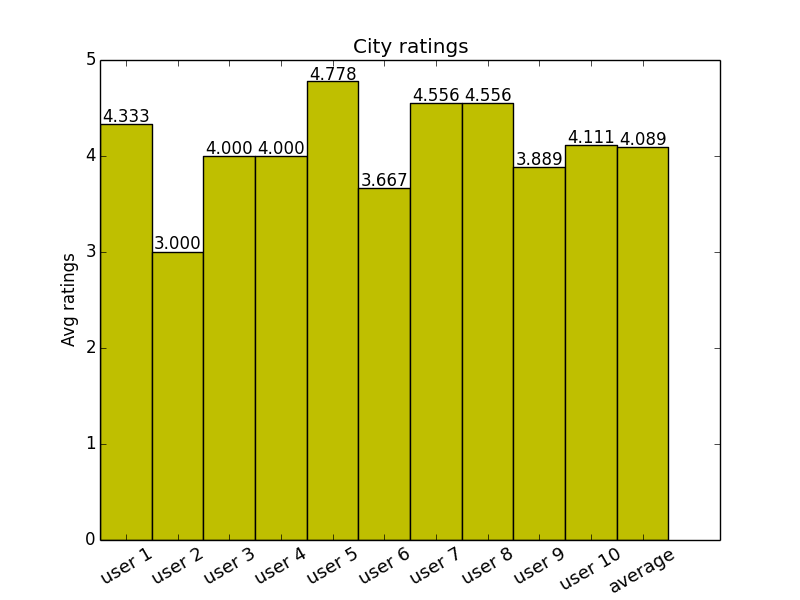
\includegraphics[width=110mm]{images/evaluation/average_city_score.png}
\caption{User average rating for city}
\label{fig:city}
\end{figure}

\begin{figure}[H]
\centering
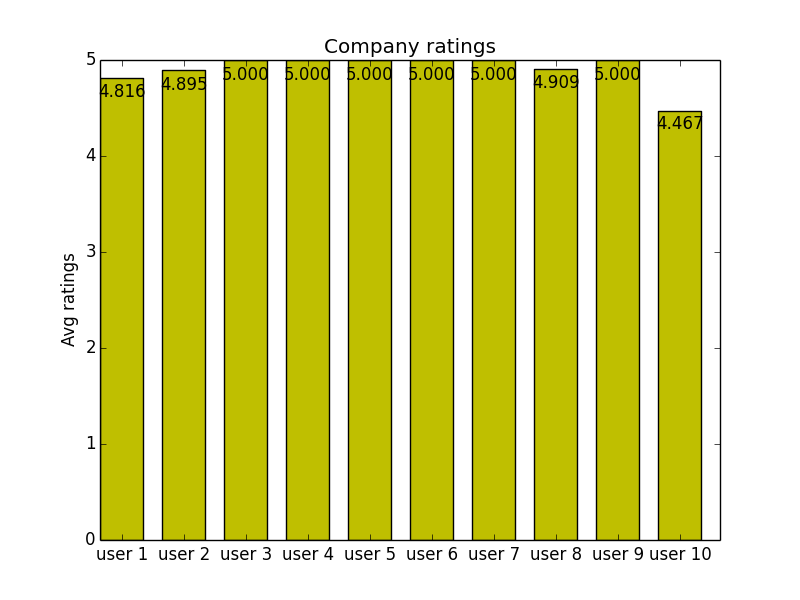
\includegraphics[width=110mm]{images/evaluation/average_company_score.png}
\caption{User average rating for company name}
\label{fig:company}
\end{figure}

\begin{figure}[H]
\centering
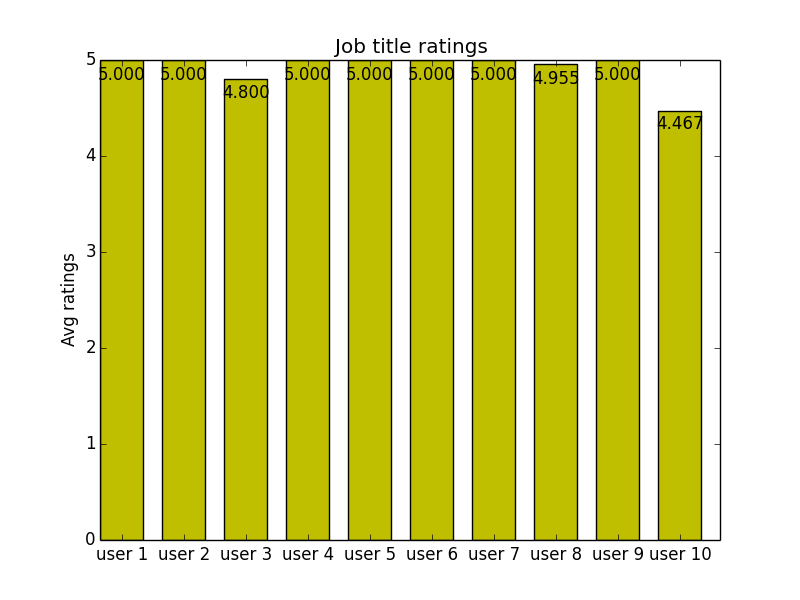
\includegraphics[width=110mm]{images/evaluation/average_job_title_score.png}
\caption{User average rating for job title}
\label{fig:job_title}
\end{figure}

\begin{figure}[H]
\centering
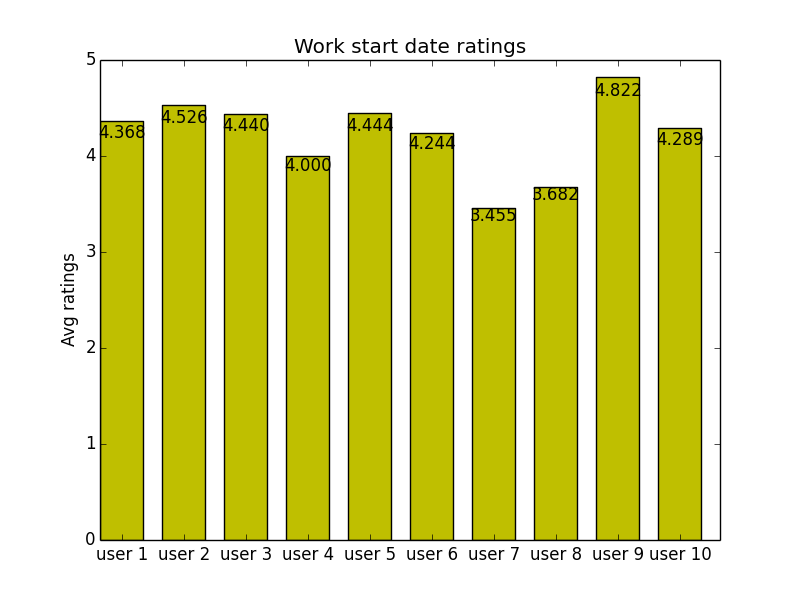
\includegraphics[width=110mm]{images/evaluation/average_experience_start_date_score.png}
\caption{User average rating for experience start data}
\label{fig:experiencestart}
\end{figure}

\begin{figure}[H]
\centering
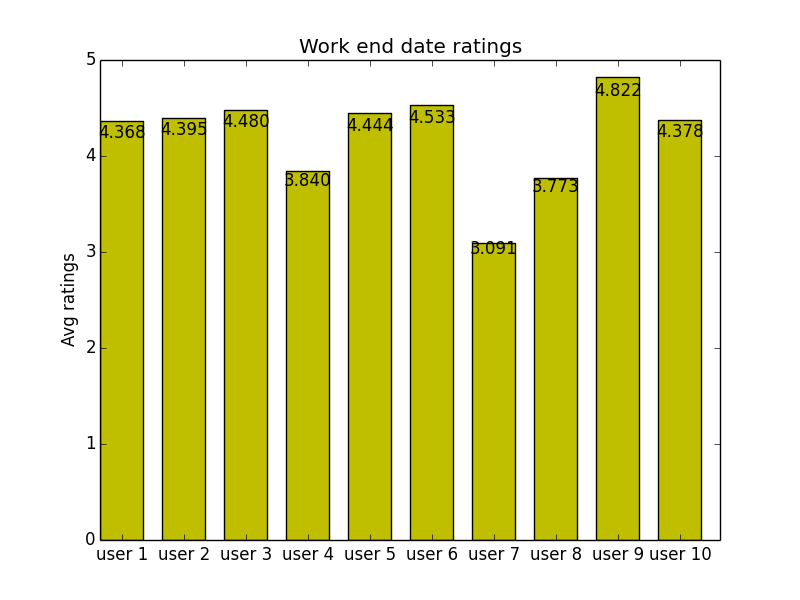
\includegraphics[width=110mm]{images/evaluation/average_experience_end_date_score.png}
\caption{User average rating for experience end data}
\label{fig:experienceend}
\end{figure}

\begin{figure}[H]
\centering
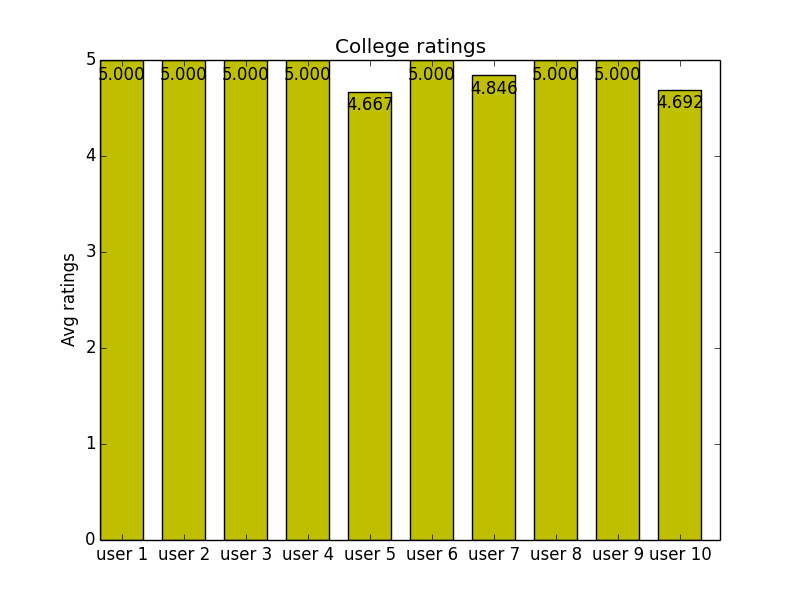
\includegraphics[width=110mm]{images/evaluation/average_college_score.png}
\caption{User average rating for college}
\label{fig:college}
\end{figure}

\begin{figure}[H]
\centering
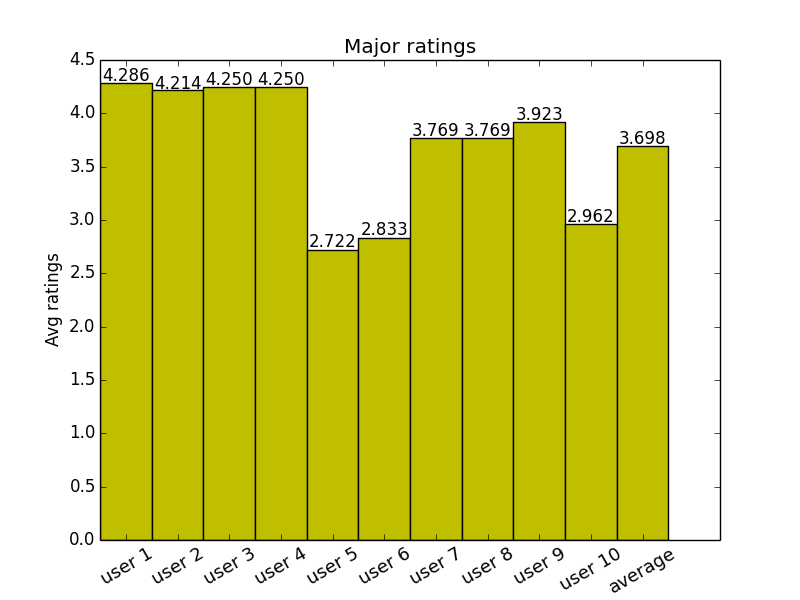
\includegraphics[width=110mm]{images/evaluation/average_major_score.png}
\caption{User average rating for major}
\label{fig:major}
\end{figure}

\begin{figure}[H]
\centering
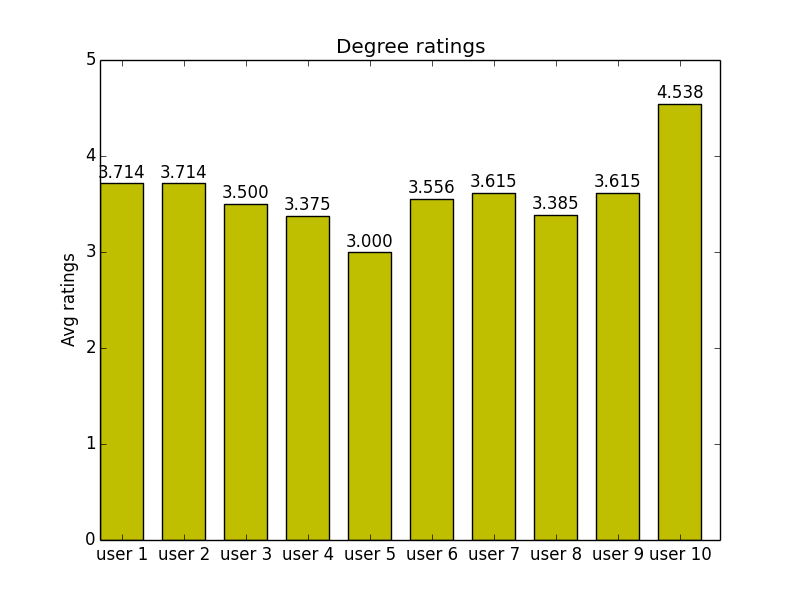
\includegraphics[width=110mm]{images/evaluation/average_degree_score.png}
\caption{User average rating for degree}
\label{fig:degree}
\end{figure}

\begin{figure}[H]
\centering
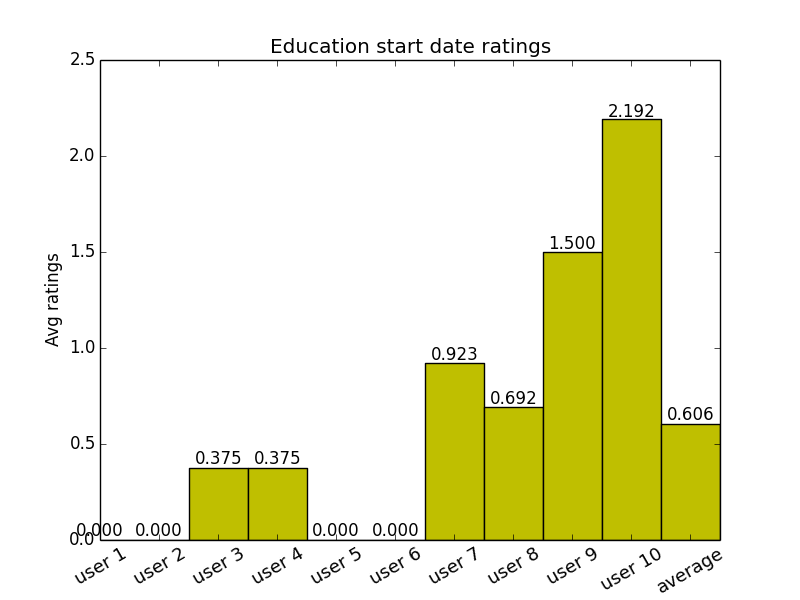
\includegraphics[width=110mm]{images/evaluation/average_education_start_date_score.png}
\caption{User average rating for education start data}
\label{fig:educationstart}
\end{figure}

\begin{figure}[H]
\centering
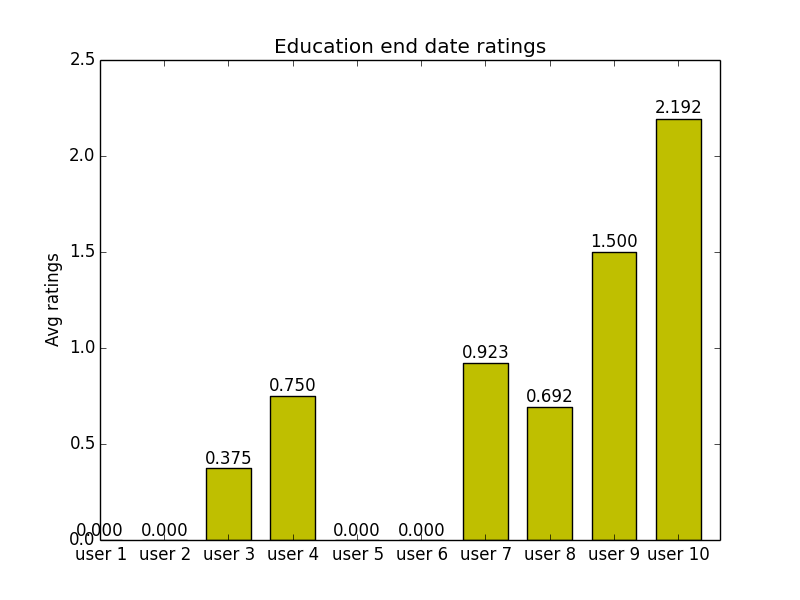
\includegraphics[width=110mm]{images/evaluation/average_education_end_date_score.png}
\caption{User average rating for education end data}
\label{fig:educationend}
\end{figure}

\subsection{Metadata fitness}

This section is a reflection on how the extracted triples fit to the data visualisation interface. The interface is divided into 3 scenarios: 

\begin{description}
	\item Scenario 1, Government \hfill \\
	The first scenario is that the interface should reflect the needs of Government officers. The fields that used by them are: city, industry type, academic degree and company size.
	\item Scenario 2, Company's human resource department \hfill \\
	The user interface also support daily queries from HR. The fields that used in this scenario are: city, degree, skill, work experience and start date.
	\item Scenario 3, Job seekers and college students
	This part allows users get insights about the employment status by city. The fields that used in this scenario are: city, degree, skill and position.
\end{description}

During the development and evaluation, we found there're some drawbacks of the extracted data that makes the query and the user interface hard to develop and use:
\begin{enumerate}
	\item Do not have information to group similar job title together. This is important as we want our query return more correct result and in the meantime keeps the query as simple as possible. For example, when one querying ``software engineer'' similar terms such as ``application developer, Java software engineer'' should all return as these job titles have no significant difference if we want to compare this job in IT over another industry. Doing this classification is hard, we will discuss 
	\item Company names may have aliases. One example is ``Oracle'' and ``Oracle EMEA''. But since we cannot find company names database as ground truth, our system cannot handle this problem. This issue is very similar to the previous one, it needs we have very accurate ground truth.
	\item As SPARQL has very limit function in datetime manipulation, the start date and end date approach in our model is not working really well. For example, if one user is looking for ``How many people had been working in a company for more then 5 years?''. The query is very hard to write so it would be easier if our model have ``year between'' field that address this requirement.
\end{enumerate}

The details of possible solution of drawbacks will be discussed in next chapter, future works section.

\section{System performance}

In \autoref{subsec:env}, we list our software and hardware details. Here we want to show the performance of some critical modules, to provide more comprehensive details of the system. One important things to know is that the performance measurements does not include database accessing and file serialisation and other miscellaneous, therefore, in production environment, the system performance could be less than the result we got.

\subsection{Parsing performance}
We run our parser 10 times, each time it parses 100 randomly selected profiles, the average time spending on parsing 100 profiles is: 18.27 seconds.

\subsection{Normalising and converting performance}
We run our RDF converter 10 times, each time in try to normalise the data in 100 profiles and convert it into RDF triples, the average time spending on this is: 345.53 seconds.

\newacronym{io}{IO}{input & output}
\subsection{Query performance}
We tried several queries with different level of complexity. Because some simple queries (for example, returning all triples) are simple but it takes a very long time on File \acrshort{io}, so we manually set ``soft limit'' equals to 2000 for each query. The ``soft limit'' means the maximum number of rows returned is 2000. Below is server case and the corresponding time:

\subsubsection{Simple query that only return subject, predicate and object}
\begin{verbatimtab}
	select * where {?subject ?predicate ?object. }
\end{verbatimtab}
The time spend on this query is: 0.548360s, and it returned 2000 rows.

\subsubsection{Simple query that asks from subject, predicate and object then summing up the subject}
\begin{verbatimtab}
	select (count(?subject) as ?total) where  {
		?subject ?predicate ?object. 
	}
\end{verbatimtab}
The time spend on this query is: 0.021132s, and it returned 1 rows.
Notice that this query is 27 times faster that the previous query even though the complexity is higher. We don't know the implementation of 4store, but one possible explaination is that the COUNT method can be optimised so the program do not really need read 2000 rows to get the actually result.

\subsubsection{A query that defines two relationships}
\begin{verbatimtab}
	select * where {
		?person a foaf:Person;
			lk:skill ?skill.
	}
\end{verbatimtab}
The time spend on this query is: 0.134334s, and it returned 2000 rows.
It is an interesting result because getting graph patterns is actually quicker than the first query, which only ask for all triples. One possible answer is the 4store SPARQL engine has special optimisation on graph matching.

\subsubsection{A query that defines two relationships with group by and count}
\begin{verbatimtab}
	select ?city (count(?person) as ?pCount) where {
		?person a foaf:Person ;
			dbpedia-owl:city ?city .
	} group by ?city
\end{verbatimtab}
The time spend on this query is: 0.011658s, and it returned 18 rows.
This time, data aggregation query is actually quicker than simple ``print all'' query. This result demonstrate 4store implementation of data aggregation has very high performance.

\subsubsection{A query that defines two relationships with group by, count and order by}
\begin{verbatimtab}
	select ?skill (count(?skill) as ?sCount) where{
		?p a foaf:Person;
			lk:skill ?skill.
	} group by ?skill order by desc(?sCount)
\end{verbatimtab}
The time spend on this query is: 7.770524s, and it returned 16184 rows.
This query takes very long time to execute. That is because to generate the correct result, the SPARQL engine has to split all the skill into groups and sum them up, there's no optimisation even we specify soft limit equals to 2000.

\subsubsection{Conclusion}
We can see that for complex group by, count and order by query, our system takes too long time to respond. One important factor that result in slow queries is the system hardware. Because we test the performance in production environment, the machine is an Amazon EC2 m1.medium instance. The hardware parameters are listed at \autoref{subsec:env}. If we can upgrade our server to high performance CPU instance, the problem should went away.

\section{Contributions}
\subsection{Reusable knowledge model from LinkedIn public profiles}
As shown in Figure~\ref{fig:KnowledgeModel}, we present a queryable, extendable knowledge graph that capture the data relationship of LinkedIn.com public profiles and company profiles. It can be used by LinkedIn internally or by other researchers who also interested in user generated content in LinkedIn.com.

\subsection{Public online SPARQL endpoint for complex query about Irish industry}
We publish our SPARQL endpoint at \url{http://goo.gl/5HyziV}. It's a standard SPARQL endpoint that powered by 4store\cite{harris20094store}. Our endpoint accept HTTP POST requests and support a number of RDF format, such as XML, JSON, plain and turtle. Anyone who interested in discover Irish industry and college facts can use this service.

\subsection{Scalable crawling strategy}
The crawling strategy is scalable to any numbers of LinkedIn public profiles. If we consider a profile is a node, since in the profile, LinkedIn will suggest 6 to 8 similar profiles (nodes), the graph is expanding very quickly (exponential increase). Therefore, data mining practitioners (and other researchers) can make use of our strategy, as discussed in \autoref{chap:impl}, to download profiles in any subdomains of LinkedIn.

\subsection{Mashup based city information extraction strategy}

Based on our user study, the strategy is widely accepted by our survey participants, with average of 0.85 F-score and 4.089/5 user rating. The approach can be generalise to get city information by company names. Another approach is to use Google reverse Geocoding service\footnote{\url{https://developers.google.com/maps/documentation/javascript/geocoding?csw=1\#ReverseGeocoding}}. However, even we don't have comparison result on hand, the result provided by reverse geocoding service seems to worse than using a country's yellowpage database.